\newpage
\chapter{Direct Simulation Monte Carlo (DSMC) Method}

The DSMC method was first proposed by Graeme Bird \cite{bird1994molecular}. This method is particularly useful for flows where the Knudsen number is past the continuum regime. This method is widely used in Micro Electro Mechanical Systems (MEMS) and the Space Shuttle's re-entry aerodynamics. \\

\no DMSC models fluid flows using probabilistic simulation molecules to solve the Boltzmann equation. Being a probabilistic algorithm that considers a set of particles rather than a single particle, it is much more computationally efficient in comparison to Molecular Dynamics. However, this very property of DSMC also makes it susceptible to statistical fluctuation in the solutions.

\section{The Algorithm}

Like any other system consisting of particles, the state of the system is given by the positions and velocities of the particles $\{ \vec{r_i}, \vec{v_i} \}$ where $i = 1, 2, 3, \cdots, N$ where $N$ is the number of simulated particles in the flow. Each simulated particle corresponds to $F_N$ physical particles with approximately the same positions and velocities. In other words, the volume $V$ of the system is given by,

\begin{equation}
	V = \frac{F_N N}{n}
\end{equation}

\no where $n$ is the number density of the flow. \\

\no The evolution of the system is obtained by integrating several properties in time steps $\tau$ usually lesser than the mean collision time $t_o$. This choice is not arbitrary. It is made with the intention of capturing all the physical phenomena with reasonable accuracy. In the absence of external force fields, the particles move ballistically,

\begin{equation}
	\vec{r}_i(t + \tau) = \vec{r}_i(t) + \vec{v}_i(t) \cdot \tau
\end{equation}

\no If and when a particle reaches a particular boundary, its position and velocity are reset according to the boundary condition applied. Once all the particles have been moved according to their velocities and positions, they are put into cells within which they randomly collide with each other based on the collision rates obtained from the \textit{Kinetic Theory of Gases}. After colliding, the velocities of the particles are reset. Statistical sampling is performed and the process is repeated. The entire process is represented in Figure \ref{img:algo}.

\begin{figure}[H]
  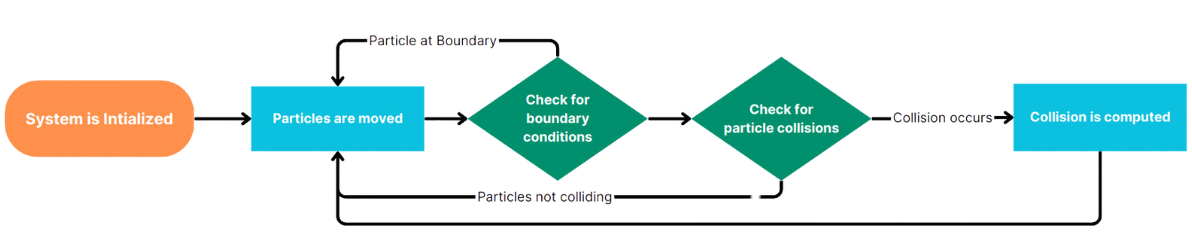
\includegraphics[scale=0.38]{Pictures/Chapter_3_DSMC/Algorithm.png}
  \centering
  \caption{Flowchart explaining a simple DSMC Algorithm}
  \label{img:algo}
\end{figure}

\section{Collisions}

Typically, when we select the dimensions of the collision grid cells, they must be no larger than the mean free path $\lambda$. This is to ensure that we get accurate collision statistics in every time step. In methods like Molecular Dynamics, two particles are not considered for a collision if their trajectories are not going to intersect. In DSMC however, all particles within a grid cell are collision candidates regardless of their actual trajectories. \\

\no There are several models that describe the collision between any two particles. The \textbf{hard spheres model}, for instance, gives the collision probability for a pair of particles $i$ and $j$ as proportional to their relative speed as,

\begin{equation}
	P_{coll}[i, j] = \frac{|\vec{v}_i - \vec{v}_j|}{\Sigma_{m=1}^{N_c} \Sigma_{n=1}^{m-1} |\vec{v}_m - \vec{v}_n|}
\end{equation}

\no where $N_c$ is the number of particles in the cell. \\

\no The double summation in the denominator can be computationally intensive, so DSMC uses a technique called \textit{rejection sampling} to select collision pairs. The steps for rejection sampling are highlighted below : -

\begin{enumerate}
	\item A pair of candidates particles $i$, $j$ is chosen at random, and their relative velocity magnitude is computed
	\item The pair is accepted as a collision pair if $v_r > v_{r_{max}} \times \mathcal{R}$ where $\mathcal{R}$ is a uniform random number in $[0,1)$.
	\item If the pair of particles are accepted, their velocities are reset but their positions are unchanged.
\end{enumerate}

\no After a collision pair is chosen, the post-collision velocities $v_i^\ast$ and $v_j^\ast$ are evaluated. The relative velocity is often conveniently expressed in terms of the spherical angles $\theta$ and $\phi$ and is given by,

\begin{equation}
	\vec{v}^\ast_r = v_r \left[ (sin\theta cos\phi) \hat{x} + (sin\theta sin\phi) \hat{y} + cos\theta \hat{z} \right]
\end{equation}

\no and these angles are selected by some Monte Carlo processes with distributions given by the selected collision model. For the hard spheres model, these angles are uniformly distributed over the unit sphere. The azimuthal angle is between $0$ and $2\pi$, and is written as $ \phi = 2\pi \mathcal{R}_1 $ where $\mathcal{R}_1$ is a uniform deviate in $[0,1)$. The polar angle is distributed according to,

\begin{equation}
	P_\theta (\theta) d\theta = \frac{1}{2} sin\theta d\theta
\end{equation}

\no Using the change of variables, $q = - cos\theta$, we obtain,

\begin{equation}
	P_q(q)dq = \frac{1}{2}dq
\end{equation}

\no where we can write $ q = 2 \mathcal{R}_2 - 1 $ where $ \mathcal{R}_2 $ is a uniform deviate in $ [0,1) $. \\

\no The post-collision velocities are set as given by the equation below,

\begin{equation}
	\vec{v}_i^\ast = \vec{v}_{cm}^\ast + \frac{1}{2} \vec{v}_r^\ast \qquad \vec{v}_j^\ast = \vec{v}_{cm}^\ast - \frac{1}{2} \vec{v}_r^\ast
\end{equation}

\no As we expect from the conservation of linear momentum and energy, the velocity of the centre of mass and the relative speed between the particles doesn't change. This process of computing collisions is repeated for every pair of particles. The total number of hard sphere collisions in a given cell during a timestep $\tau$ is given by,

\begin{equation}
	M_{coll} = \frac{1}{2} (N_c - 1) F_N f_{coll} \tau = \frac{N_c (N_c - 1) F_N \pi d^2 \langle v_r \rangle \tau}{2 V_c}
\end{equation}

\no where $f_{coll}$ is the collision frequency given by the Kinetic Theory of Gases, $d$ is the diameter of the cell and $V_c$ is the volume of the cell. The ratio of the total accepted to the total number of candidates for hard sphere particles are given by,

\begin{equation}
	\frac{M_{coll}}{M_{cand}} = \frac{\langle v_r \rangle}{v_r^{max}}
\end{equation}